%form: dc_form_03-04.tex ; user: dc_03-04_preparation_etc.tex
%========== DC =========
%===== p. 03-04 現在までの研究状況 =============
\section{現在までの研究状況}
%watermark: w03_past_dc
\newcommand{\研究の背景}{%
%begin  研究の背景===================
	\subsection{2.で述べた研究状況を踏まえこれからの研究計画の背景}
	\noindent
	●\textbf{2.で述べた研究状況を踏まえこれからの研究計画の背景}

	自然言語処理は、
	%前後の文脈を考慮できるBERT\cite{devlin-etal-2019-bert}や
	前節で述べたGrover\cite{NIPS2019_9106}を始め、
	より自然な文章が近年は生成できるようになった。
	前節の研究では実際にGroverを拡張し\textbf{コメントを生成することでより多くのフェイクニュースを検出}した。
	また、DNNは出力に対する説明が不足するブラックボックス問題があったが、それを解決する説明可能なモデルも開発されている\cite{shu2019defend}。
	今後は、\textbf{検出と説明の両面から実際に拡散の抑制をより期待できるモデルの開発を目指す}。

	\subsection{問題点・解決すべき点}
	\noindent
	●\textbf{問題点・解決すべき点}

	生成コメントを付加して分類した場合、前節提案モデルがFakeと判断した中で実際にFakeだった割合である精度(Precision)は0.59だった。
	これは生成コメントを付加せず分類したときの0.68と比べ0.09ポイント下回る\cite{EasyChair:3190}。
	つまり\textbf{提案モデルがFakeと判断したユニット中、41\%はRealを誤って検出した}。
	精度と再現率の調和平均であるF値(F1 score)も、提案モデルは\textbf{0.68}と良好なものではなかった。

	同時に、生成されたコメントは文法における不可解な点が多いため、生成コメントから判断の根拠とする説明可能性の提供は難しい。
	これではいくらフェイクニュースを検出できても、
	\textbf{判断の理由も説明できない狼少年めいたモデル}ではユーザの信用を得るのは難しく、拡散の抑制にはならない。

	この\textbf{分類性能不足}と、\textbf{不自然なコメントにより説明可能性を提供できない}2点を解決する必要がある。

	\subsection{着想に至った経緯}
	\noindent
	●\textbf{着想に至った経緯}

	実際に早期自動検出モデルをSNS上で運用する場合を想定した。
	このモデルの目的は拡散の抑制であるため、\textbf{フェイクニュース以上にユーザの信用を得なければ拡散を食い止められない}。
	そのためには、真偽分類の性能を上げることと、説得力向上のために説明可能性を同時に提供する必要があると着想に至った。

	{\footnotesize
		\begin{thebibliography}{99}
			\vspace*{-1mm}
			\setlength{\parskip}{0cm}
			\setlength{\itemsep}{0cm}
			\setcounter{enumiv}{7}
			\begin{spacing}{0.7}
				\bibitem{shu2019defend} Kai Shu, \textit{et al.} defend: Explainable fake news detection. In \textit{Proc. of the ACM SIGKDD}, 2019.
			\end{spacing}
			\end{thebibliography}
			
		%\bibliography{myreferences}
		%\bibliographystyle{junsrt}
	}
%end  研究の背景 ====================
}

\newcommand{\現在までの研究状況}{%
%begin  現在までの研究状況===================
	この研究では、フェイクニュースの早期自動検出のために、記事に加えてユーザのコメントを扱った。
	ただし拡散初期段階ではコメントの数が少ないため、コメントを生成・付加することで検出を補助した。
	実際にコメントを生成して真偽分類した結果、付加しない時より多くのフェイクニュースを検出した。

	\subsection{これまでの研究の背景}
	\noindent
	●\textbf{これまでの研究の背景}

	SNSの発展により、情報を迅速かつ大量に取得し、拡散することで容易に共有できるようになった。
	一方、悪意により他人を騙すために作られた\textbf{フェイクニュース}が拡散されやすくなった。
	ユーザの間で拡散されると、\textbf{誤った認識が広がって騙された人々が社会的損害を起こす}という問題があるため、
	\textbf{\underline{フェイクニュース拡散の早期抑制が必要とされている}}。
	%例えば、2016年米国大統領選挙前にフェイクニュースに騙された人々がピザ屋で銃撃事件を起こした\cite{agencies_2016}。
	%特に今年はCOVID-19にまつわるフェイクニュースが広く拡散され、不安に陥った人々が買いだめを行うことが世界的に問題となった。
	%WHOは情報の過剰な氾濫を``インフォデミック''と定義し、テドロス事務局長は\textbf{誤った情報はウイルス以上に拡散されやすい}と指摘した\cite{ZAROCOSTAS2020676}。

	\subsection{問題点}
	\noindent
	●\textbf{問題点}

	現在フェイクニュースの拡散抑制のために、有識者が事実関係の確認を行う\textbf{ファクトチェック}がとられている。
	しかしこれは(1)属人的な作業であること、(2)拡散されてから調査されることが多いこと、
	以上の理由より結果を公表するまで時間がかかる。
	このためフェイクニュースと比べ拡散されず、拡散抑制に繋がらないことが多い。
	そこで迅速なファクトチェックを行うために、ニューステキストや添付メディア、
	そしてユーザの反応からディープニューラルネットワーク (DNN)を利用しフェイクニュースを自動で検出する手法が多く開発されている
	\cite{Wang:2018:EEA:3219819.3219903}。
	特に、ユーザの反応は真偽によって大きな違いがみられる(i.e. フェイクである指摘やbotの介入)ことから、集合知として活用した研究も多くみられる\cite{Wu:2018:TFF:3159652.3159677}。
	%これを自動で検出する場合、フェイクニュースは巧妙に実際のニュースを模した形をとるため、\textbf{単純なルールベース手法では難しい}。
	%近年ではニューステキストや添付メディア、ユーザの反応から\textbf{ディープニューラルネットワーク(DNN)}を利用した手法がみられる。
	%この場合はブラックボックス問題により\textbf{説明可能性が不足}するため、SNSユーザから支持を得にくい。
	%その中で\textbf{ユーザの反応は拡散後でしか得られない}ため、早期の検出を想定した場合はユーザの反応を評価対象にすることができない。

	しかし、これらの手法において\textbf{ユーザの反応は拡散後でしか得られない}ため、早期の検出を想定した場合は評価対象が制限され自動検出の性能が落ちてしまう問題がある。

	\subsection{解決方策}
	\noindent
	●\textbf{解決方策}

	そこで本研究ではDNNの\textbf{学習でのみユーザの反応を活用}し、テスト時は\textbf{ユーザの反応をコメント生成モデルにより生成・補完}して分類することで、
	\textbf{性能を落とさず早期検出を目指す}ことにした。

	\subsection{研究目的・研究方法}
	\noindent
	●\textbf{研究目的・研究方法}

	フェイクニュース早期検出に向け、SNS上でニュースに寄せられたコメントを生成することが、
	真偽を分類するの向上につながることを明らかにする。
	本研究はニュースと寄せられたコメントを、
	ニュースの本文と実際にSNS上で投稿されたコメント3件(モデル構造とデータセットの都合上)を1ユニットとして扱うことにした。
	コメント生成と真偽分類はそれぞれモデルを独立させた。
	真偽分類においては図\ref{fig:model}のように、コメントを1件削除し学習済コメント生成モデルから1件コメントを生成し補完した。
	
	\begin{figure}[ht]
		\centering
		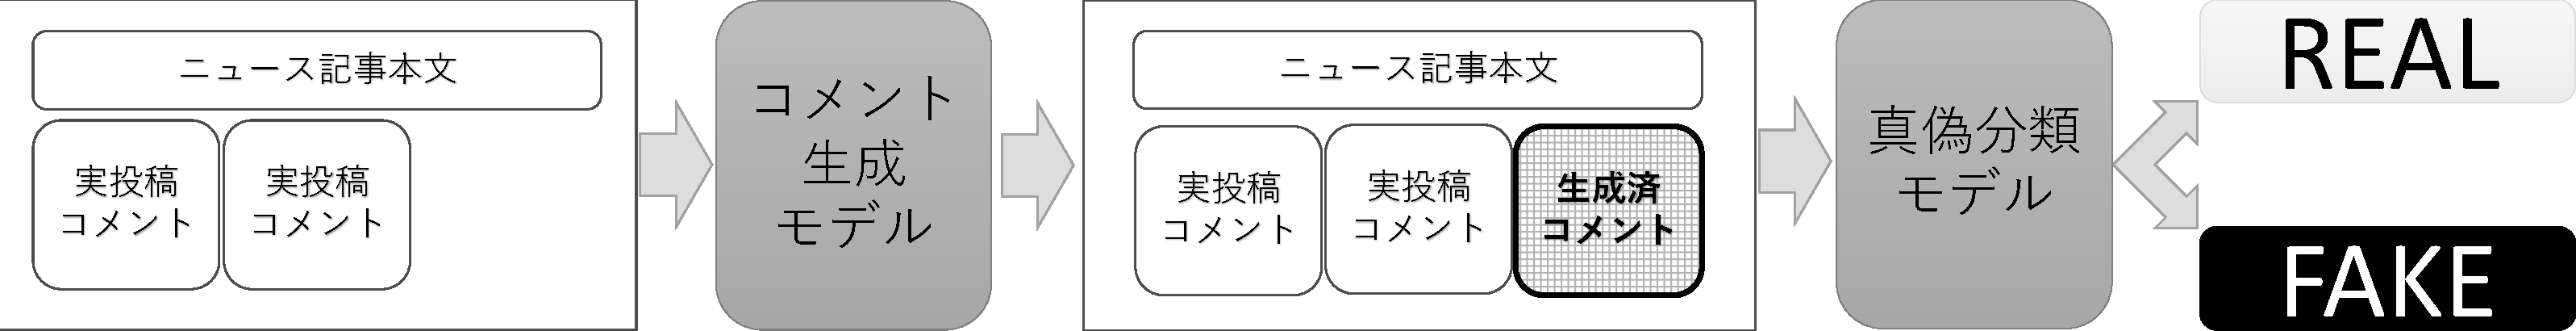
\includegraphics[width=0.95\linewidth]{figs/model.pdf}
		\vspace*{-3mm}
		\caption{提案手法の真偽判断までの流れ。}
		\label{fig:model}
	\end{figure}
	\vspace*{-4mm}
	\subsection{特色と独創的な点}
	\noindent
	●\textbf{特色と独創的な点}
	\vspace*{-3mm}
	\begin{itemize}
		\setlength{\parskip}{0cm}
		\setlength{\itemsep}{0cm}
		\item SNS上の拡散スピードに追いつくことが検出モデルのコンセプトである点
		\item \textbf{真偽を評価する分類タスクに、コメントの生成タスクを組み込んだ点}
		\item 分類性能を大きく失わずに速報性をもつことができる点
	\end{itemize}
	\vspace*{-2mm}

	特に2点目が、先行研究ではみられない本研究最大のの学術的特色であると申請者は考えている。

	\subsection{これまでの研究経過及び得られた結果}
	\noindent
	●\textbf{これまでの研究経過及び得られた結果}

	申請者はデータセットとしてFakeNewsNet\cite{Shu2018FakeNewsNetAD, shu2017fake}を使用した。
	このデータセットは、ファクトチェックで真偽が評価済である英文ニュースと、それにTwitter上で言及された投稿(ツイート)等をもつ。
	本研究では最低3件以上英文でコメントとしてツイートが寄せられた芸能ニュースを真偽で各2000件使用した。
	拡散の初期段階ではコメントの数は期待できないため、使用するコメントは各3件ずつ無作為に選出し、残りは対象から除外した。

	生成・分類モデルは、フェイクニュースを自動で作成するGroverモデル\cite{NIPS2019_9106}を拡張する形で実装した。
	このモデルはフェイクニュースをドメイン・著者・投稿日・見出し・本文の5要素に分け、\textbf{ランダムで歯抜けにして予測させる形で生成学習を実現}したものである。
	今回はこれをユニットの4要素(記事本文と3件のコメント)での実装を目指し調整を行った。
	訓練が完了したコメント生成モデルを使い、図\ref{fig:model}の通り\textbf{コメントを1件欠損させたユニットに生成コメントを付加した上で、RealかFakeか分類させた}。
	分類モデルはGroverが提供したものを流用した。

	その結果、提案モデルによって生成されたコメントを含めて分類した際、\textbf{Fake記事を見抜いた割合を示す再現率(Recall)が0.79}と、欠損のまま分類させたときの\textbf{0.75}を上回った。
	つまり、コメントを生成することで\textbf{ファクトチェックが必要な疑わしい記事をより多く検出}した\cite{EasyChair:3190}。
	%同時に、生成されたコメントで頻出した単語の傾向において真偽で大きな違いはみられなかった。
	%これは、\textbf{記事の真偽によってコメント内の単語傾向の差は軽微}であることを意味した。
	これは提案コメント生成モデルが、記事本文とコメントのみから信憑性による傾向の差異の学習に成功していることを示唆する。

	\vspace*{1mm}
	{\footnotesize 
	%\bibliography{myreferences}
	%\bibliographystyle{junsrt}
	\begin{thebibliography}{99}
		\vspace*{-2mm}
		\setlength{\parskip}{0cm}
		\setlength{\itemsep}{0cm}
		\begin{spacing}{0.7}
		%\bibitem{agencies_2016} Guardian staff and agencies. Washington gunman motivated by fake news `pizzagate' conspiracy,12 2016.
		\bibitem{ZAROCOSTAS2020676} John Zarocostas. How to fight an infodemic. \textit{The Lancet}, Vol. 395, No. 10225, p. 676, 2020.
		\bibitem{Wang:2018:EEA:3219819.3219903} Yaqing Wang, \textit{et al.} EANN: Event Adversarial Neural Networks for Multi-Modal Fake News Detection. In \textit{Proc. of KDD'18}, pp. 849-857. 2018.
		\bibitem{Wu:2018:TFF:3159652.3159677} Liang Wu and Huan Liu. Tracing Fake-News Footprints: Characterizing Social Media Messages by How They Propagate. In \textit{Proc. of WSDM '18},  pp. 637-645, 2018.
		\bibitem{Shu2018FakeNewsNetAD} Kai Shu, \textit{et al.} Fakenewsnet: Adata repository with news content, social context and dynamic information for studying fake news on social media. \textit{ArXiv}, Vol. abs/1809.01286, 2018.
		\bibitem{shu2017fake} Kai Shu, \textit{et al.} Fake News Detection on Social Media: A Data Mining Perspective. \textit{ACM SIGKDD Explorations Newsletter}, Vol. 19, No. 1, pp. 22-36, 2017.
		\bibitem{NIPS2019_9106} Rowan Zellers, \textit{et al.} Defending against neural fake news. \textit{NIPS 2019}, pp. 9054–9065, 2019.
		\bibitem{EasyChair:3190} Yuta Yanagi, \textit{et al.} Fake news detection with generated comments for news articles. \textit{EasyChair Preprint no. 3190}, EasyChair, 2020.
		\end{spacing}
	\end{thebibliography}
	}
	%ぞうの卵はおいしいぞう。
ぞうの卵はおいしいぞう。
ぞうの卵はおいしいぞう。
ぞうの卵はおいしいぞう。
ぞうの卵はおいしいぞう。
ぞうの卵はおいしいぞう。
ぞうの卵はおいしいぞう。
ぞうの卵はおいしいぞう。
ぞうの卵はおいしいぞう。
ぞうの卵はおいしいぞう。
ぞうの卵はおいしいぞう。
ぞうの卵はおいしいぞう。
ぞうの卵はおいしいぞう。
ぞうの卵はおいしいぞう。
ぞうの卵はおいしいぞう。
ぞうの卵はおいしいぞう。
ぞうの卵はおいしいぞう。
ぞうの卵はおいしいぞう。
ぞうの卵はおいしいぞう。
ぞうの卵はおいしいぞう。
ぞうの卵はおいしいぞう。
ぞうの卵はおいしいぞう。
ぞうの卵はおいしいぞう。
ぞうの卵はおいしいぞう。
ぞうの卵はおいしいぞう。
ぞうの卵はおいしいぞう。
ぞうの卵はおいしいぞう。
ぞうの卵はおいしいぞう。
ぞうの卵はおいしいぞう。
ぞうの卵はおいしいぞう。
ぞうの卵はおいしいぞう。
ぞうの卵はおいしいぞう。
ぞうの卵はおいしいぞう。
ぞうの卵はおいしいぞう。
ぞうの卵はおいしいぞう。
ぞうの卵はおいしいぞう。
ぞうの卵はおいしいぞう。
ぞうの卵はおいしいぞう。
ぞうの卵はおいしいぞう。
ぞうの卵はおいしいぞう。
ぞうの卵はおいしいぞう。
ぞうの卵はおいしいぞう。
ぞうの卵はおいしいぞう。
ぞうの卵はおいしいぞう。
ぞうの卵はおいしいぞう。
ぞうの卵はおいしいぞう。
ぞうの卵はおいしいぞう。
ぞうの卵はおいしいぞう。
ぞうの卵はおいしいぞう。
ぞうの卵はおいしいぞう。
ぞうの卵はおいしいぞう。
ぞうの卵はおいしいぞう。
ぞうの卵はおいしいぞう。
ぞうの卵はおいしいぞう。
ぞうの卵はおいしいぞう。
ぞうの卵はおいしいぞう。
ぞうの卵はおいしいぞう。
ぞうの卵はおいしいぞう。
ぞうの卵はおいしいぞう。
ぞうの卵はおいしいぞう。
ぞうの卵はおいしいぞう。
ぞうの卵はおいしいぞう。
ぞうの卵はおいしいぞう。
ぞうの卵はおいしいぞう。
ぞうの卵はおいしいぞう。
ぞうの卵はおいしいぞう。
ぞうの卵はおいしいぞう。
ぞうの卵はおいしいぞう。
ぞうの卵はおいしいぞう。
ぞうの卵はおいしいぞう。
ぞうの卵はおいしいぞう。
ぞうの卵はおいしいぞう。
ぞうの卵はおいしいぞう。
ぞうの卵はおいしいぞう。
ぞうの卵はおいしいぞう。
ぞうの卵はおいしいぞう。
ぞうの卵はおいしいぞう。
ぞうの卵はおいしいぞう。
ぞうの卵はおいしいぞう。
ぞうの卵はおいしいぞう。
ぞうの卵はおいしいぞう。
ぞうの卵はおいしいぞう。
ぞうの卵はおいしいぞう。
ぞうの卵はおいしいぞう。
ぞうの卵はおいしいぞう。
ぞうの卵はおいしいぞう。
ぞうの卵はおいしいぞう。
ぞうの卵はおいしいぞう。
ぞうの卵はおいしいぞう。
ぞうの卵はおいしいぞう。
ぞうの卵はおいしいぞう。
ぞうの卵はおいしいぞう。
ぞうの卵はおいしいぞう。
ぞうの卵はおいしいぞう。
ぞうの卵はおいしいぞう。
ぞうの卵はおいしいぞう。
ぞうの卵はおいしいぞう。
ぞうの卵はおいしいぞう。
ぞうの卵はおいしいぞう。
ぞうの卵はおいしいぞう。
ぞうの卵はおいしいぞう。
ぞうの卵はおいしいぞう。
ぞうの卵はおいしいぞう。
ぞうの卵はおいしいぞう。
ぞうの卵はおいしいぞう。
ぞうの卵はおいしいぞう。
ぞうの卵はおいしいぞう。
ぞうの卵はおいしいぞう。
ぞうの卵はおいしいぞう。
ぞうの卵はおいしいぞう。
ぞうの卵はおいしいぞう。
ぞうの卵はおいしいぞう。
ぞうの卵はおいしいぞう。
ぞうの卵はおいしいぞう。
ぞうの卵はおいしいぞう。
ぞうの卵はおいしいぞう。
ぞうの卵はおいしいぞう。
ぞうの卵はおいしいぞう。
ぞうの卵はおいしいぞう。
ぞうの卵はおいしいぞう。
ぞうの卵はおいしいぞう。
ぞうの卵はおいしいぞう。
ぞうの卵はおいしいぞう。
ぞうの卵はおいしいぞう。
ぞうの卵はおいしいぞう。
ぞうの卵はおいしいぞう。
ぞうの卵はおいしいぞう。
ぞうの卵はおいしいぞう。
ぞうの卵はおいしいぞう。
ぞうの卵はおいしいぞう。
ぞうの卵はおいしいぞう。
ぞうの卵はおいしいぞう。
ぞうの卵はおいしいぞう。
ぞうの卵はおいしいぞう。
ぞうの卵はおいしいぞう。
ぞうの卵はおいしいぞう。
ぞうの卵はおいしいぞう。
ぞうの卵はおいしいぞう。
ぞうの卵はおいしいぞう。
ぞうの卵はおいしいぞう。
ぞうの卵はおいしいぞう。
ぞうの卵はおいしいぞう。
ぞうの卵はおいしいぞう。
ぞうの卵はおいしいぞう。
ぞうの卵はおいしいぞう。
ぞうの卵はおいしいぞう。
ぞうの卵はおいしいぞう。
ぞうの卵はおいしいぞう。
ぞうの卵はおいしいぞう。
ぞうの卵はおいしいぞう。
ぞうの卵はおいしいぞう。
ぞうの卵はおいしいぞう。
ぞうの卵はおいしいぞう。
ぞうの卵はおいしいぞう。
ぞうの卵はおいしいぞう。
ぞうの卵はおいしいぞう。
ぞうの卵はおいしいぞう。
  % << only for demonstration. Please delete it or comment it out.	
%end  現在までの研究状況 ====================
}

